%\documentclass{standalone}
%\usepackage{tikz}
%\usetikzlibrary{patterns,plotmarks}
%\begin{document}
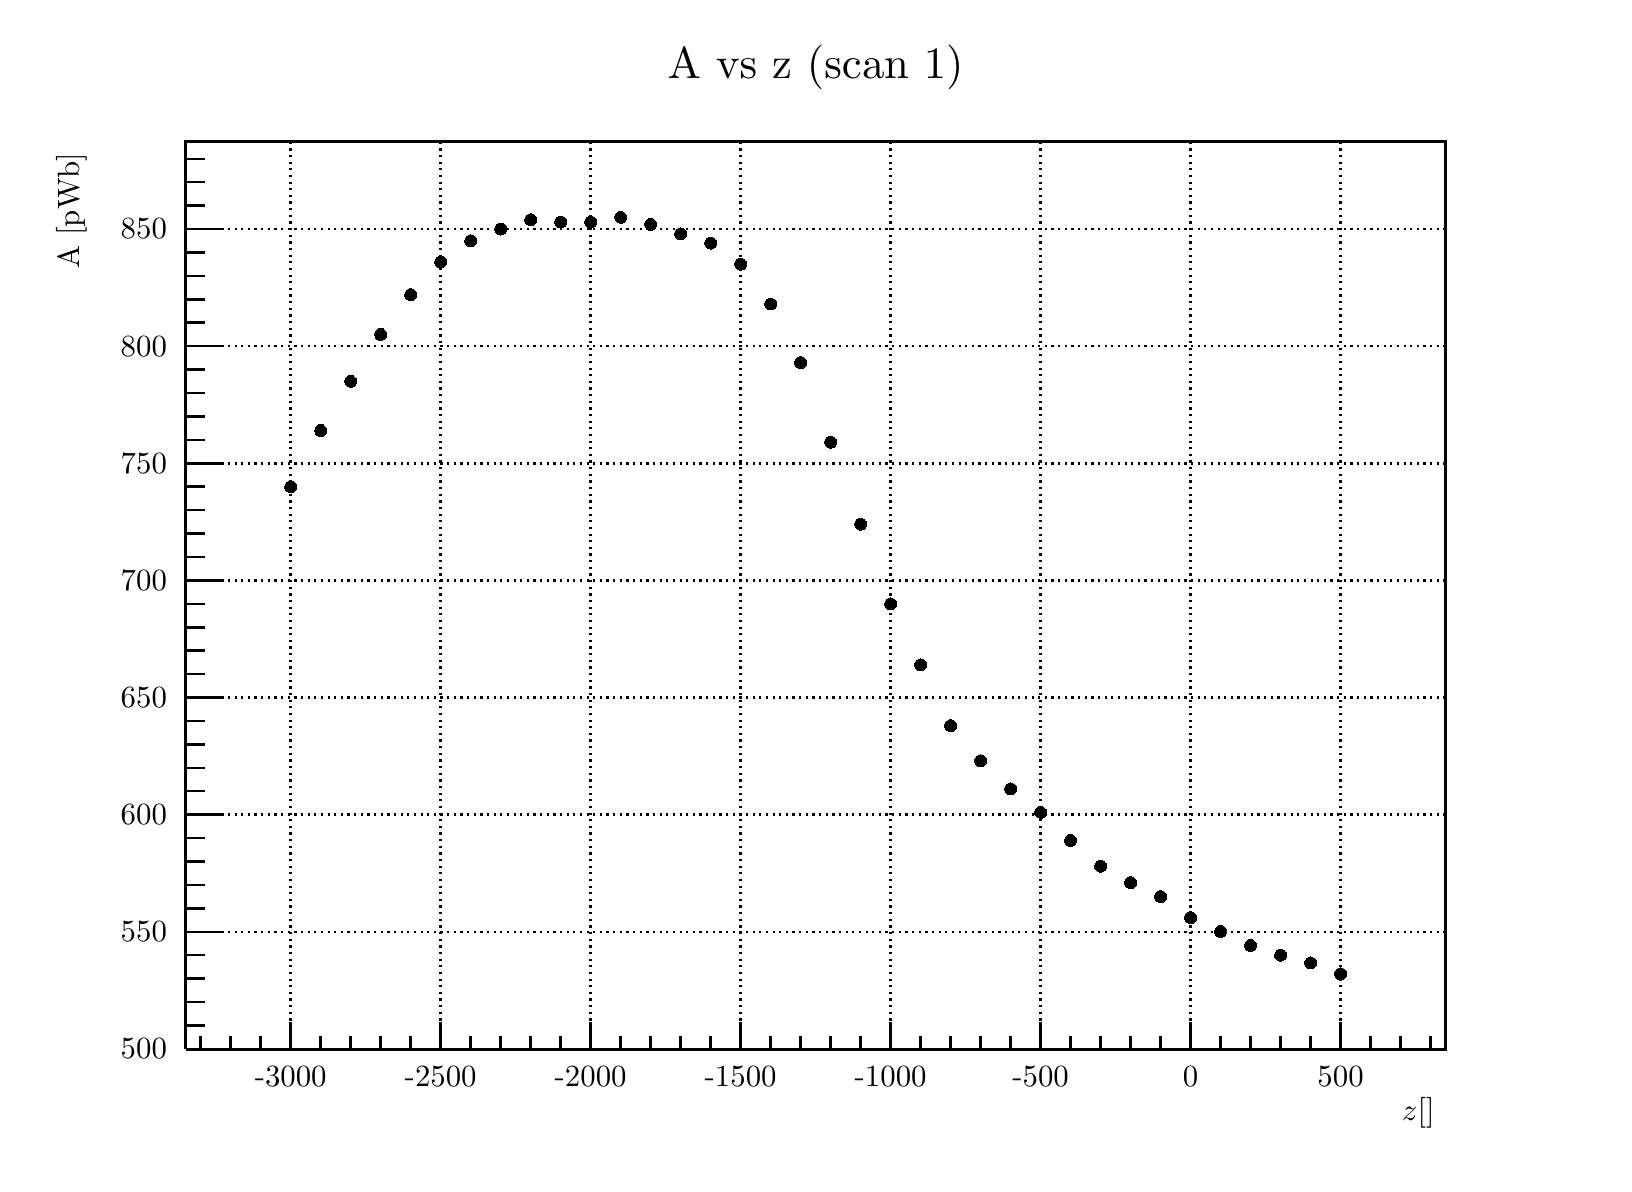
\begin{tikzpicture}
\def\CheckTikzLibraryLoaded#1{ \ifcsname tikz@library@#1@loaded\endcsname \else \PackageWarning{tikz}{usetikzlibrary{#1} is missing in the preamble.} \fi }
\CheckTikzLibraryLoaded{patterns}
\CheckTikzLibraryLoaded{plotmarks}
\pgfdeclareplotmark{cross} {
\pgfpathmoveto{\pgfpoint{-0.3\pgfplotmarksize}{\pgfplotmarksize}}
\pgfpathlineto{\pgfpoint{+0.3\pgfplotmarksize}{\pgfplotmarksize}}
\pgfpathlineto{\pgfpoint{+0.3\pgfplotmarksize}{0.3\pgfplotmarksize}}
\pgfpathlineto{\pgfpoint{+1\pgfplotmarksize}{0.3\pgfplotmarksize}}
\pgfpathlineto{\pgfpoint{+1\pgfplotmarksize}{-0.3\pgfplotmarksize}}
\pgfpathlineto{\pgfpoint{+0.3\pgfplotmarksize}{-0.3\pgfplotmarksize}}
\pgfpathlineto{\pgfpoint{+0.3\pgfplotmarksize}{-1.\pgfplotmarksize}}
\pgfpathlineto{\pgfpoint{-0.3\pgfplotmarksize}{-1.\pgfplotmarksize}}
\pgfpathlineto{\pgfpoint{-0.3\pgfplotmarksize}{-0.3\pgfplotmarksize}}
\pgfpathlineto{\pgfpoint{-1.\pgfplotmarksize}{-0.3\pgfplotmarksize}}
\pgfpathlineto{\pgfpoint{-1.\pgfplotmarksize}{0.3\pgfplotmarksize}}
\pgfpathlineto{\pgfpoint{-0.3\pgfplotmarksize}{0.3\pgfplotmarksize}}
\pgfpathclose
\pgfusepathqstroke
}
\pgfdeclareplotmark{cross*} {
\pgfpathmoveto{\pgfpoint{-0.3\pgfplotmarksize}{\pgfplotmarksize}}
\pgfpathlineto{\pgfpoint{+0.3\pgfplotmarksize}{\pgfplotmarksize}}
\pgfpathlineto{\pgfpoint{+0.3\pgfplotmarksize}{0.3\pgfplotmarksize}}
\pgfpathlineto{\pgfpoint{+1\pgfplotmarksize}{0.3\pgfplotmarksize}}
\pgfpathlineto{\pgfpoint{+1\pgfplotmarksize}{-0.3\pgfplotmarksize}}
\pgfpathlineto{\pgfpoint{+0.3\pgfplotmarksize}{-0.3\pgfplotmarksize}}
\pgfpathlineto{\pgfpoint{+0.3\pgfplotmarksize}{-1.\pgfplotmarksize}}
\pgfpathlineto{\pgfpoint{-0.3\pgfplotmarksize}{-1.\pgfplotmarksize}}
\pgfpathlineto{\pgfpoint{-0.3\pgfplotmarksize}{-0.3\pgfplotmarksize}}
\pgfpathlineto{\pgfpoint{-1.\pgfplotmarksize}{-0.3\pgfplotmarksize}}
\pgfpathlineto{\pgfpoint{-1.\pgfplotmarksize}{0.3\pgfplotmarksize}}
\pgfpathlineto{\pgfpoint{-0.3\pgfplotmarksize}{0.3\pgfplotmarksize}}
\pgfpathclose
\pgfusepathqfillstroke
}
\pgfdeclareplotmark{newstar} {
\pgfpathmoveto{\pgfqpoint{0pt}{\pgfplotmarksize}}
\pgfpathlineto{\pgfqpointpolar{44}{0.5\pgfplotmarksize}}
\pgfpathlineto{\pgfqpointpolar{18}{\pgfplotmarksize}}
\pgfpathlineto{\pgfqpointpolar{-20}{0.5\pgfplotmarksize}}
\pgfpathlineto{\pgfqpointpolar{-54}{\pgfplotmarksize}}
\pgfpathlineto{\pgfqpointpolar{-90}{0.5\pgfplotmarksize}}
\pgfpathlineto{\pgfqpointpolar{234}{\pgfplotmarksize}}
\pgfpathlineto{\pgfqpointpolar{198}{0.5\pgfplotmarksize}}
\pgfpathlineto{\pgfqpointpolar{162}{\pgfplotmarksize}}
\pgfpathlineto{\pgfqpointpolar{134}{0.5\pgfplotmarksize}}
\pgfpathclose
\pgfusepathqstroke
}
\pgfdeclareplotmark{newstar*} {
\pgfpathmoveto{\pgfqpoint{0pt}{\pgfplotmarksize}}
\pgfpathlineto{\pgfqpointpolar{44}{0.5\pgfplotmarksize}}
\pgfpathlineto{\pgfqpointpolar{18}{\pgfplotmarksize}}
\pgfpathlineto{\pgfqpointpolar{-20}{0.5\pgfplotmarksize}}
\pgfpathlineto{\pgfqpointpolar{-54}{\pgfplotmarksize}}
\pgfpathlineto{\pgfqpointpolar{-90}{0.5\pgfplotmarksize}}
\pgfpathlineto{\pgfqpointpolar{234}{\pgfplotmarksize}}
\pgfpathlineto{\pgfqpointpolar{198}{0.5\pgfplotmarksize}}
\pgfpathlineto{\pgfqpointpolar{162}{\pgfplotmarksize}}
\pgfpathlineto{\pgfqpointpolar{134}{0.5\pgfplotmarksize}}
\pgfpathclose
\pgfusepathqfillstroke
}
\definecolor{c}{rgb}{1,1,1};
\draw [color=c, fill=c] (0,0) rectangle (20,14.411);
\draw [color=c, fill=c] (2,1.4411) rectangle (18,12.9699);
\definecolor{c}{rgb}{0,0,0};
\draw [c,line width=0.9] (2,1.4411) -- (2,12.9699) -- (18,12.9699) -- (18,1.4411) -- (2,1.4411);
\definecolor{c}{rgb}{1,1,1};
\draw [color=c, fill=c] (2,1.4411) rectangle (18,12.9699);
\definecolor{c}{rgb}{0,0,0};
\draw [c,line width=0.9] (2,1.4411) -- (2,12.9699) -- (18,12.9699) -- (18,1.4411) -- (2,1.4411);
\draw [c,line width=0.9] (2,1.4411) -- (18,1.4411);
\draw [c,dash pattern=on 0.80pt off 1.60pt ,line width=0.9] (3.33333,12.9699) -- (3.33333,1.4411);
\draw [c,dash pattern=on 0.80pt off 1.60pt ,line width=0.9] (5.2381,12.9699) -- (5.2381,1.4411);
\draw [c,dash pattern=on 0.80pt off 1.60pt ,line width=0.9] (7.14286,12.9699) -- (7.14286,1.4411);
\draw [c,dash pattern=on 0.80pt off 1.60pt ,line width=0.9] (9.04762,12.9699) -- (9.04762,1.4411);
\draw [c,dash pattern=on 0.80pt off 1.60pt ,line width=0.9] (10.9524,12.9699) -- (10.9524,1.4411);
\draw [c,dash pattern=on 0.80pt off 1.60pt ,line width=0.9] (12.8571,12.9699) -- (12.8571,1.4411);
\draw [c,dash pattern=on 0.80pt off 1.60pt ,line width=0.9] (14.7619,12.9699) -- (14.7619,1.4411);
\draw [c,dash pattern=on 0.80pt off 1.60pt ,line width=0.9] (16.6667,12.9699) -- (16.6667,1.4411);
\draw [c,dash pattern=on 0.80pt off 1.60pt ,line width=0.9] (3.33333,12.9699) -- (3.33333,1.4411);
\draw [c,dash pattern=on 0.80pt off 1.60pt ,line width=0.9] (16.6667,12.9699) -- (16.6667,1.4411);
\draw [c,line width=0.9] (2,1.4411) -- (2,12.9699);
\draw [c,dash pattern=on 0.80pt off 1.60pt ,line width=0.9] (18,1.44839) -- (2,1.44839);
\draw [c,dash pattern=on 0.80pt off 1.60pt ,line width=0.9] (18,2.93583) -- (2,2.93583);
\draw [c,dash pattern=on 0.80pt off 1.60pt ,line width=0.9] (18,4.42326) -- (2,4.42326);
\draw [c,dash pattern=on 0.80pt off 1.60pt ,line width=0.9] (18,5.9107) -- (2,5.9107);
\draw [c,dash pattern=on 0.80pt off 1.60pt ,line width=0.9] (18,7.39814) -- (2,7.39814);
\draw [c,dash pattern=on 0.80pt off 1.60pt ,line width=0.9] (18,8.88557) -- (2,8.88557);
\draw [c,dash pattern=on 0.80pt off 1.60pt ,line width=0.9] (18,10.373) -- (2,10.373);
\draw [c,dash pattern=on 0.80pt off 1.60pt ,line width=0.9] (18,11.8604) -- (2,11.8604);
\draw [c,dash pattern=on 0.80pt off 1.60pt ,line width=0.9] (18,1.44839) -- (2,1.44839);
\draw [c,dash pattern=on 0.80pt off 1.60pt ,line width=0.9] (18,11.8604) -- (2,11.8604);
\draw [c,line width=0.9] (2,1.4411) -- (18,1.4411);
\draw [c,line width=0.9] (3.33333,1.78697) -- (3.33333,1.4411);
\draw [c,line width=0.9] (3.71429,1.61404) -- (3.71429,1.4411);
\draw [c,line width=0.9] (4.09524,1.61404) -- (4.09524,1.4411);
\draw [c,line width=0.9] (4.47619,1.61404) -- (4.47619,1.4411);
\draw [c,line width=0.9] (4.85714,1.61404) -- (4.85714,1.4411);
\draw [c,line width=0.9] (5.2381,1.78697) -- (5.2381,1.4411);
\draw [c,line width=0.9] (5.61905,1.61404) -- (5.61905,1.4411);
\draw [c,line width=0.9] (6,1.61404) -- (6,1.4411);
\draw [c,line width=0.9] (6.38095,1.61404) -- (6.38095,1.4411);
\draw [c,line width=0.9] (6.7619,1.61404) -- (6.7619,1.4411);
\draw [c,line width=0.9] (7.14286,1.78697) -- (7.14286,1.4411);
\draw [c,line width=0.9] (7.52381,1.61404) -- (7.52381,1.4411);
\draw [c,line width=0.9] (7.90476,1.61404) -- (7.90476,1.4411);
\draw [c,line width=0.9] (8.28571,1.61404) -- (8.28571,1.4411);
\draw [c,line width=0.9] (8.66667,1.61404) -- (8.66667,1.4411);
\draw [c,line width=0.9] (9.04762,1.78697) -- (9.04762,1.4411);
\draw [c,line width=0.9] (9.42857,1.61404) -- (9.42857,1.4411);
\draw [c,line width=0.9] (9.80952,1.61404) -- (9.80952,1.4411);
\draw [c,line width=0.9] (10.1905,1.61404) -- (10.1905,1.4411);
\draw [c,line width=0.9] (10.5714,1.61404) -- (10.5714,1.4411);
\draw [c,line width=0.9] (10.9524,1.78697) -- (10.9524,1.4411);
\draw [c,line width=0.9] (11.3333,1.61404) -- (11.3333,1.4411);
\draw [c,line width=0.9] (11.7143,1.61404) -- (11.7143,1.4411);
\draw [c,line width=0.9] (12.0952,1.61404) -- (12.0952,1.4411);
\draw [c,line width=0.9] (12.4762,1.61404) -- (12.4762,1.4411);
\draw [c,line width=0.9] (12.8571,1.78697) -- (12.8571,1.4411);
\draw [c,line width=0.9] (13.2381,1.61404) -- (13.2381,1.4411);
\draw [c,line width=0.9] (13.619,1.61404) -- (13.619,1.4411);
\draw [c,line width=0.9] (14,1.61404) -- (14,1.4411);
\draw [c,line width=0.9] (14.381,1.61404) -- (14.381,1.4411);
\draw [c,line width=0.9] (14.7619,1.78697) -- (14.7619,1.4411);
\draw [c,line width=0.9] (15.1429,1.61404) -- (15.1429,1.4411);
\draw [c,line width=0.9] (15.5238,1.61404) -- (15.5238,1.4411);
\draw [c,line width=0.9] (15.9048,1.61404) -- (15.9048,1.4411);
\draw [c,line width=0.9] (16.2857,1.61404) -- (16.2857,1.4411);
\draw [c,line width=0.9] (16.6667,1.78697) -- (16.6667,1.4411);
\draw [c,line width=0.9] (3.33333,1.78697) -- (3.33333,1.4411);
\draw [c,line width=0.9] (2.95238,1.61404) -- (2.95238,1.4411);
\draw [c,line width=0.9] (2.57143,1.61404) -- (2.57143,1.4411);
\draw [c,line width=0.9] (2.19048,1.61404) -- (2.19048,1.4411);
\draw [c,line width=0.9] (16.6667,1.78697) -- (16.6667,1.4411);
\draw [c,line width=0.9] (17.0476,1.61404) -- (17.0476,1.4411);
\draw [c,line width=0.9] (17.4286,1.61404) -- (17.4286,1.4411);
\draw [c,line width=0.9] (17.8095,1.61404) -- (17.8095,1.4411);
\draw [anchor=base] (3.33333,0.965539) node[scale=1.11327, color=c, rotate=0]{-3000};
\draw [anchor=base] (5.2381,0.965539) node[scale=1.11327, color=c, rotate=0]{-2500};
\draw [anchor=base] (7.14286,0.965539) node[scale=1.11327, color=c, rotate=0]{-2000};
\draw [anchor=base] (9.04762,0.965539) node[scale=1.11327, color=c, rotate=0]{-1500};
\draw [anchor=base] (10.9524,0.965539) node[scale=1.11327, color=c, rotate=0]{-1000};
\draw [anchor=base] (12.8571,0.965539) node[scale=1.11327, color=c, rotate=0]{-500};
\draw [anchor=base] (14.7619,0.965539) node[scale=1.11327, color=c, rotate=0]{0};
\draw [anchor=base] (16.6667,0.965539) node[scale=1.11327, color=c, rotate=0]{500};
\draw [anchor= east] (18,0.634085) node[scale=1.11327, color=c, rotate=0]{$z [\mum]$};
\draw [c,line width=0.9] (2,1.4411) -- (2,12.9699);
\draw [c,line width=0.9] (2.48,1.44839) -- (2,1.44839);
\draw [c,line width=0.9] (2.24,1.74588) -- (2,1.74588);
\draw [c,line width=0.9] (2.24,2.04337) -- (2,2.04337);
\draw [c,line width=0.9] (2.24,2.34085) -- (2,2.34085);
\draw [c,line width=0.9] (2.24,2.63834) -- (2,2.63834);
\draw [c,line width=0.9] (2.48,2.93583) -- (2,2.93583);
\draw [c,line width=0.9] (2.24,3.23331) -- (2,3.23331);
\draw [c,line width=0.9] (2.24,3.5308) -- (2,3.5308);
\draw [c,line width=0.9] (2.24,3.82829) -- (2,3.82829);
\draw [c,line width=0.9] (2.24,4.12578) -- (2,4.12578);
\draw [c,line width=0.9] (2.48,4.42326) -- (2,4.42326);
\draw [c,line width=0.9] (2.24,4.72075) -- (2,4.72075);
\draw [c,line width=0.9] (2.24,5.01824) -- (2,5.01824);
\draw [c,line width=0.9] (2.24,5.31573) -- (2,5.31573);
\draw [c,line width=0.9] (2.24,5.61321) -- (2,5.61321);
\draw [c,line width=0.9] (2.48,5.9107) -- (2,5.9107);
\draw [c,line width=0.9] (2.24,6.20819) -- (2,6.20819);
\draw [c,line width=0.9] (2.24,6.50568) -- (2,6.50568);
\draw [c,line width=0.9] (2.24,6.80316) -- (2,6.80316);
\draw [c,line width=0.9] (2.24,7.10065) -- (2,7.10065);
\draw [c,line width=0.9] (2.48,7.39814) -- (2,7.39814);
\draw [c,line width=0.9] (2.24,7.69562) -- (2,7.69562);
\draw [c,line width=0.9] (2.24,7.99311) -- (2,7.99311);
\draw [c,line width=0.9] (2.24,8.2906) -- (2,8.2906);
\draw [c,line width=0.9] (2.24,8.58809) -- (2,8.58809);
\draw [c,line width=0.9] (2.48,8.88557) -- (2,8.88557);
\draw [c,line width=0.9] (2.24,9.18306) -- (2,9.18306);
\draw [c,line width=0.9] (2.24,9.48055) -- (2,9.48055);
\draw [c,line width=0.9] (2.24,9.77804) -- (2,9.77804);
\draw [c,line width=0.9] (2.24,10.0755) -- (2,10.0755);
\draw [c,line width=0.9] (2.48,10.373) -- (2,10.373);
\draw [c,line width=0.9] (2.24,10.6705) -- (2,10.6705);
\draw [c,line width=0.9] (2.24,10.968) -- (2,10.968);
\draw [c,line width=0.9] (2.24,11.2655) -- (2,11.2655);
\draw [c,line width=0.9] (2.24,11.563) -- (2,11.563);
\draw [c,line width=0.9] (2.48,11.8604) -- (2,11.8604);
\draw [c,line width=0.9] (2.48,1.44839) -- (2,1.44839);
\draw [c,line width=0.9] (2.48,11.8604) -- (2,11.8604);
\draw [c,line width=0.9] (2.24,12.1579) -- (2,12.1579);
\draw [c,line width=0.9] (2.24,12.4554) -- (2,12.4554);
\draw [c,line width=0.9] (2.24,12.7529) -- (2,12.7529);
\draw [anchor= east] (1.9,1.44839) node[scale=1.11327, color=c, rotate=0]{500};
\draw [anchor= east] (1.9,2.93583) node[scale=1.11327, color=c, rotate=0]{550};
\draw [anchor= east] (1.9,4.42326) node[scale=1.11327, color=c, rotate=0]{600};
\draw [anchor= east] (1.9,5.9107) node[scale=1.11327, color=c, rotate=0]{650};
\draw [anchor= east] (1.9,7.39814) node[scale=1.11327, color=c, rotate=0]{700};
\draw [anchor= east] (1.9,8.88557) node[scale=1.11327, color=c, rotate=0]{750};
\draw [anchor= east] (1.9,10.373) node[scale=1.11327, color=c, rotate=0]{800};
\draw [anchor= east] (1.9,11.8604) node[scale=1.11327, color=c, rotate=0]{850};
\draw [anchor= east] (0.54812,12.9699) node[scale=1.11327, color=c, rotate=90]{A [pWb]};
\foreach \P in {(3.33333,8.58809), (3.71429,9.30206), (4.09524,9.92678), (4.47619,10.5218), (4.85714,11.0275), (5.2381,11.444), (5.61905,11.7117), (6,11.8604), (6.38095,11.9794), (6.7619,11.9497), (7.14286,11.9497), (7.52381,12.0092),
 (7.90476,11.9199), (8.28571,11.8009), (8.66667,11.682), (9.04762,11.4142), (9.42857,10.9085), (9.80952,10.1648), (10.1905,9.15331), (10.5714,8.11211), (10.9524,7.10065), (11.3333,6.32718), (11.7143,5.55372), (12.0952,5.10748), (12.4762,4.7505),
 (12.8571,4.45301), (13.2381,4.09603), (13.619,3.76879), (14,3.56055), (14.381,3.38206), (14.7619,3.11551), (15.1429,2.94029), (15.5238,2.7618), (15.9048,2.63864), (16.2857,2.54076), (16.6667,2.40184)}{\draw[mark options={color=c,fill=c},mark
 size=2.162162pt, line width=0.000000pt, mark=*] plot coordinates {\P};}
\draw (10,13.9179) node[scale=1.61424, color=c, rotate=0]{A vs z (scan 1)};
\end{tikzpicture}
%\end{document}
